% LaTeX source for textbook ``ThinkCPP , a game perspective''
% Copyright (C) 2023  Lisa Patacchiola and Allen B. Downey


\chapter{The way of the program}

The goal of this book is to teach you to think like a
computer scientist.  I like the way computer scientists think because
they combine some of the best features of Mathematics, Engineering,
and Natural Science.  Like mathematicians, computer scientists use formal
languages to denote ideas (specifically computations).  Like
engineers, they design things, assembling components into systems and
evaluating trade-offs among alternatives.  Like scientists,
they observe the behavior of complex systems, form hypotheses, and test
predictions.

The single most important skill for a computer scientist is {\bf
problem-solving}.  By that I mean the ability to formulate problems,
think creatively about solutions, and express a solution clearly and
accurately.  As it turns out, the process of learning to program is an
excellent opportunity to practice problem-solving skills.  That's why
this chapter is called ``The way of the program.''

\section{What is a programming language?}
\index{programming language}
\index{language!programming}

The programming language you will be learning is C++, because it is used 
in many video games and in the Unreal Engine. Both C++ and C\# are
 {\bf high-level languages}; other high-level languages you might have 
heard of are Java, C and Python.

As you might infer from the name ``high-level language,'' there are
also {\bf low-level languages}, sometimes referred to as machine
language or assembly language.  Loosely-speaking, computers can only
execute programs written in low-level languages.  Thus, programs
written in a high-level language have to be translated before they can
run.  This translation takes some time, which is a small disadvantage
of high-level languages.

\index{portability}
\index{high-level language}
\index{low-level language}
\index{language!high-level}
\index{language!low-level}

But the advantages are enormous.  First,
it is {\em much} easier to program in a high-level language;
by ``easier'' I mean that the program takes less time to write,
it's shorter and easier to read, and it's more likely to be
correct.  Secondly, high-level languages are {\bf portable},
meaning that they can run on different kinds of computers with
few or no modifications.  Low-level programs can only run
on one kind of computer, and have to be rewritten to run on
another.

Due to these advantages, almost all programs are written in
high-level languages.  Low-level languages are only used for
a few special applications.

\index{compile}
\index{interpret}

There are two ways to translate a program; {\bf interpreting} or {\bf
compiling}.  An interpreter is a program that reads a high-level
program and does what it says.  In effect, it translates the program
line-by-line, alternately reading lines and carrying out commands.

\vspace{0.1in}
\begin{figure}[h]
    \centering
    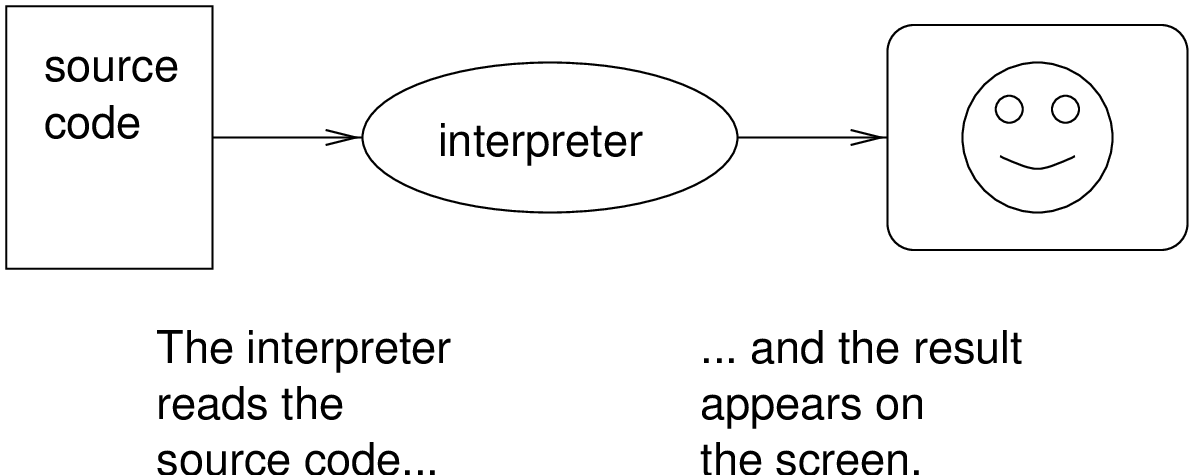
\includegraphics[width=9cm]{oldimages/interpret.png}
    \caption{From source code to Result}
    \label{fig:throughinterpret}
\end{figure}
\vspace{0.1in}

A compiler is a program that reads a high-level program and
translates it all at once, before executing any of the commands.
Often you compile the program as a separate step, and then
execute the compiled code later.  In this case, the high-level
program is called the {\bf source code}, and the translated
program is called the {\bf object code} or the {\bf executable}.

As an example, suppose you write a program in C++.  You might
use a text editor to write the program (a text editor is
a simple word processor).  When the program is finished, you
might save it in a file named {\tt program.cpp}, where ``program''
is an arbitrary name you make up, and the suffix {\tt .cpp} is
a convention that indicates that the file contains C++ source
code.

Then, depending on what your programming environment is like,
you might leave the text editor and run the compiler.  The
compiler would read your source code, translate it, and create
a new file named {\tt program.o} or {\tt program.obj} to contain the object code,
and {\tt program.out} or {\tt program.exe} to contain the executable. 

\vspace{0.1in}
\centerline{\epsfig{figure=oldimages/compile.eps}}
\vspace{0.1in}

The next step is to run the program, which requires some kind
of executor.  The role of the executor is to load the program
(copy it from disk into memory) and make the computer start
executing the program.

Although this process may seem complicated, the good news is that in
most programming environments (sometimes called integrated development
environments(IDE)), these steps are automated for you.  Usually you will
only have to write a program and type a single command to compile and
run it.  On the other hand, it is useful to know what the steps are
that are happening in the background so that if something goes wrong,
you can figure out what it is.

\index{replit}
The longer code examples in this book will use Replit.com, an online programming
platform/IDE, and community. Code listings include links to the “repl” that you can copy 
(“fork”) and experiment with.

\section{What is a program?}

A program is a sequence of instructions that specifies how to perform
a computation.  The computation might be something mathematical, like
solving a system of equations or finding the roots of a polynomial,
but it can also be a symbolic computation, like searching and
replacing text in a document or (strangely enough) compiling a
program. Or, it could be something fun, like a character trying to walk around and find a dragon. All of these things can be done with a program.

\index{statement}

The instructions (or commands, or statements) look different in
different programming languages, but there are a few basic functions
that appear in just about every language:

\begin{description}
\item[input:] Get data from the keyboard, or a file, or some
other device.

\item[output:] Display data on the screen or send data to a
file or other device.

\item[math:] Perform basic mathematical operations like addition and
multiplication. (Sometimes called "Processing")

\item[testing:] Check for certain conditions and execute the
appropriate sequence of statements. (Sometimes called "Selection")

\item[repetition:] Perform some action repeatedly, usually with
some variation. (Sometimes called "Iteration" or "looping")

\index{input}
\index{output}
\index{math}
\index{processing}
\index{testing}
\index{selection}
\index{iteration}
\index{repetition}
\index{loop}

\end{description}

Believe it or not, that's pretty much all there is to it.
Every program you've ever used, no matter how complicated, is
made up of functions that look more or less like these.  Thus,
one way to describe programming is the process of breaking a
large, complex task up into smaller and smaller subtasks
until eventually the subtasks are simple enough to be performed
with one of these simple functions.

\section{What is debugging?}
\index{debugging}
\index{bug}

Programming is a complex process, and since it is done by
human beings, it often leads to errors.  For whimsical reasons,
programming errors are called {\bf bugs} and the process
of tracking them down and correcting them is called
{\bf debugging}.

There are a few different kinds of errors that can occur
in a program, and it is useful to distinguish between them
in order to track them down more quickly.

\subsection{Compile-time errors}
\index{compile-time error}
\index{error!compile-time}
\index{error!syntax}
\index{syntax error}

The compiler can only translate a program if the program is
syntactically correct; otherwise, the compilation fails and
you will not be able to run your program.  {\bf Syntax}
refers to the structure of your program and the rules about
that structure. A mistake with the syntax is often called a {\bf syntax error}.

\index{syntax}

For example, in English, a sentence must begin with a capital
letter and end with a period.  this sentence contains a syntax
error.  So does this one

For most readers, a few syntax errors are not a significant
problem, which is why we can read the poetry of e e cummings
without spewing error messages.

Compilers are not so forgiving.  If there is a single syntax
error anywhere in your program, the compiler will print an
error message and quit, and you will not be able to run
your program.

To make matters worse, there are more syntax rules in C++
than there are in English, and the error messages you get from
the compiler are often not very helpful.  During the first
few weeks of your programming career, you will probably
spend a lot of time tracking down syntax errors.  As you
gain experience, though, you will make fewer errors and find
them faster.

When you get a syntax error, don't think that the compiler is yelling at you for getting something wrong. Think of it ask asking you for help. "Help" it is saying "I have no idea what this means, please help me". Honestly, I like syntax errors more than any of the other types of errors. Syntax errors are one of the few errors where the computer tells you it found a problem and suggests what it thinks is wrong. 
\subsection{Run-time errors}
\label{run-time}
\index{run-time error}
\index{error!run-time}
\index{safe language}
\index{language!safe}

The second type of error is a run-time error, so-called because
the error does not appear until you run the program.

For the simple sorts of programs we will be writing for the
next few weeks, run-time errors are rare, so it might be a little
while before you encounter one.


\subsection{Logic errors and semantics}
\index{semantics}
\index{logic error}
\index{error!logic}

The third type of error is the {\bf logical} or {\bf semantic}
error.  If there is a logical error in your program, it will
compile and run successfully, in the sense that the computer
will not generate any error messages, but it will not do the
right thing.  It will do something else.  Specifically, it will
do what you told it to do.

The problem is that the program you wrote is not the program
you wanted to write.  The meaning of the program (its semantics)
is wrong.  

Let's say you have a program that tells the computer to do the following steps:
\begin{enumerate}
    \item Get the pitcher of water
    \item Pour the water
    \item Get the glass
\end{enumerate}
A person would see that list and would assume you meant to get the glass first. The computer would do exactly as you asked and spill water on the table and then put a glass on top. There was an obvious logical error in your program, but it ran without a compile error. As far as the computer was concerned, it ran perfectly. But, you know that was not your original intent.

Identifying logical errors can be tricky, since
it requires you to work backwards by looking at the output
of the program and trying to figure out what it is doing.

\subsection{Experimental debugging}

One of the most important skills you should acquire from working with
this book is debugging.  Although it can be frustrating, debugging is
one of the most intellectually rich, challenging, and interesting
parts of programming.

In some ways debugging is like detective work.  You are
confronted with clues and you have to infer the processes
and events that lead to the results you see.

Debugging is also like an experimental science.  Once you have an idea
what is going wrong, you modify your program and try again.  If your
hypothesis was correct, then you can predict the result of the
modification, and you take a step closer to a working program.  If
your hypothesis was wrong, you have to come up with a new one.  As
Sherlock Holmes pointed out, ``When you have eliminated the
impossible, whatever remains, however improbable, must be the truth.''
(from A. Conan Doyle's {\em The Sign of Four}).

\index{Holmes, Sherlock}
\index{Doyle, Arthur Conan}

For some people, programming and debugging are the
same thing.  That is, programming is the process of gradually
debugging a program until it does what you want.  The idea
is that you should always start with a working program that
does {\em something}, and make small modifications, debugging
them as you go, so that you always have a working program.

For example, Linux is an operating system that contains thousands of
lines of code, but it started out as a simple program Linus Torvalds
used to explore the Intel 80386 chip.  According to Larry Greenfield,
``One of Linus's earlier projects was a program that would switch
between printing AAAA and BBBB.  This later evolved to Linux''
(from {\em The Linux Users' Guide} Beta Version 1).

\index{Linux}

In later chapters I will make more suggestions about debugging
and other programming practices.

\section{Formal and natural languages}
\label{formal}
\index{formal language}
\index{natural language}
\index{language!formal}
\index{language!natural}

{\bf Natural languages} are the languages that people speak,
like English, Spanish, and French.  They were not designed
by people (although people try to impose some order on them);
they evolved naturally.

{\bf Formal languages} are languages that are designed by people for
specific applications.  For example, the notation that mathematicians
use is a formal language that is particularly good at denoting
relationships among numbers and symbols.  Chemists use a formal
language to represent the chemical structure of molecules.  And
most importantly:

\begin{quote}
{\bf Programming languages are formal languages that have been
designed to express computations.}
\end{quote}

As I mentioned before, formal languages tend to have strict rules
about syntax.  For example, $3+3=6$ is a syntactically correct
mathematical statement, but $3=+6\$$ is not.  Also, $H_2O$ is a
syntactically correct chemical name, but $_2Zz$ is not.

Syntax rules come in two flavors, pertaining to tokens and structure.
Tokens are the basic elements of the language, like words and numbers
and chemical elements.  One of the problems with {\tt 3=+6\$} is that
{\tt \$} is not a legal token in mathematics (at least as far as I
know).  Similarly, $_2Zz$ is not legal because there is no element with
the abbreviation $Zz$.

The second type of syntax error pertains to the structure of a
statement; that is, the way the tokens are arranged.  The statement
{\tt 3=+6\$} is structurally illegal, because you can't have a plus
sign immediately after an equals sign.  Similarly, molecular formulas
have to have subscripts after the element name, not before.

When you read a sentence in English or a statement in a formal
language, you have to figure out what the structure of the sentence is
(although in a natural language you do this unconsciously).  This
process is called {\bf parsing}.

\index{parse}

For example, when you hear the sentence, ``The other shoe fell,'' you
understand that ``the other shoe'' is the subject and ``fell'' is the
verb.  Once you have parsed a sentence, you can figure out what it
means, that is, the semantics of the sentence.  Assuming that you know
what a shoe is, and what it means to fall, you will understand the
general implication of this sentence.

Although formal and natural languages have many features in
common---tokens, structure, syntax and semantics---there are many
differences.

\index{ambiguity}
\index{redundancy}
\index{literalness}

\begin{description}

\item[ambiguity:] Natural languages are full of ambiguity, which
people deal with by using contextual clues and other information.
Formal languages are designed to be nearly or completely unambiguous,
which means that any statement has exactly one meaning,
regardless of context.

\item[redundancy:] In order to make up for ambiguity and reduce
misunderstandings, natural languages employ lots of
redundancy.  As a result, they are often verbose.  Formal languages
are less redundant and more concise.

\item[literalness:] Natural languages are full of idiom and
metaphor.  If I say, ``The other shoe fell,'' there is probably
no shoe and nothing falling.  Formal languages mean
exactly what they say.

\end{description}

People who grow up speaking a natural language (everyone) often have a
hard time adjusting to formal languages.  In some ways the difference
between formal and natural language is like the difference between
poetry and prose, but more so:

\index{poetry}
\index{prose}

\begin{description}

\item[Poetry:] Words are used for their sounds as well as for
their meaning, and the whole poem together creates an effect or
emotional response.  Ambiguity is not only common but often
deliberate.

\item[Prose:] The literal meaning of words is more important
and the structure contributes more meaning.  Prose is more amenable to
analysis than poetry, but still often ambiguous.

\item[Programs:] The meaning of a computer program is unambiguous
and literal, and can be understood entirely by analysis of the
tokens and structure.

\end{description}

Here are some suggestions for reading programs (and other formal
languages).  First, remember that formal languages are much more dense
than natural languages, so it takes longer to read them.  Also, the
structure is very important, so it is usually not a good idea to read
from top to bottom, left to right.  Instead, learn to parse the
program in your head, identifying the tokens and interpreting the
structure.  Finally, remember that the details matter.  Little things
like spelling errors and bad punctuation, which you can get away
with in natural languages, can make a big difference in a formal
language.

\section{The first program}
\label{hello}
\index{hello world}

Traditionally the first program people write in a new language
is called ``Hello, World.'' because all it does is print the
words ``Hello, World.''  In C++, this program looks like this:


\begin{lstlisting}[frame=single]
#include <iostream>

// main: generate some simple output

int main ()
{
  std::cout << "Hello, world." << std::endl;
  return 0;
}
\end{lstlisting}
%

Some people judge the quality of a programming language by
the simplicity of the ``Hello, World.'' program.  By this
standard, C++ does reasonably well.  Even so, this simple
program contains several features that are hard to explain to
beginning programmers.  For now, we will ignore some of
them, like the first line.

\index{comment}
\index{statement!comment}

The third line begins with {\tt //}, which indicates
that it is a {\bf comment}.  A comment is a bit of
English text that you can put in the middle of a program,
usually to explain what the program does.  When the compiler
sees a {\tt //}, it ignores everything from there until the end
of the line.

In the fourth line, you can ignore the word {\tt int}
for now, but notice the word {\tt main}.  {\tt main} is a
special name that indicates the place in the program where execution
begins.  When the program runs, it starts by executing the first
statement in {\tt main} and it continues, in order, until it gets
to the last statement, and then it quits.

\index{output}
\index{statement!output}

There is no limit to the number of statements that can be in {\tt
main}, but the example contains only one.  It is a basic {\bf
output} statement, meaning that it outputs or displays a message on
the screen.  

{\tt std::cout} is a special object provided by the system to allow
you to send output to the screen.  The symbol {\tt <<} is an
{\bf operator} that you apply to {\tt std::cout} and a string, and that
causes the string to be displayed.

\index{operator}

{\tt std::endl} is a special symbol that represents the end of a
line.  When you send an {\tt std::endl} to {\tt std::cout}, it causes the
cursor to move to the next line of the display.
The next time you output something, the new text appears
on the next line. (Note: the word is endl ends with an L, not a 1.)

Like all statements, the output statement ends with a
semi-colon ({\tt ;}).

There are a few other things you should notice about the syntax of
this program.  First, C++ uses curly-braces (\{ and
\}) to group things together.  In this case, the output statement
is enclosed in curly-braces, indicating that it is {\em inside} the
definition of {\tt main}.  Also, notice that the statement is
indented, which helps to show visually which lines are inside the
definition.

At this point it would be a good idea to sit down in front of
a computer and compile and run this program.  

To try program out, go to:
\href{https://replit.com/@lpatacch/helloWorld#hello.cpp}{Hello World Project}.

\index{replit}
When the project is loaded, you should see a button that looks like Figure \ref{fig:Run}.
\smallskip
\begin{figure}
    \centering
    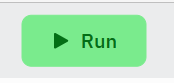
\includegraphics{Run}
    \caption{The Run button on Replit}
    \label{fig:Run}
\end{figure}

If you click that "Run" button, it will compile the code and run it. You should see the words "Hello World!" on the right side of the environment. Congratulations! You just created your first program!

As I mentioned, the C++ compiler is a real stickler for syntax.
If you make any errors when you type in the program, chances
are that it will not compile successfully.  For example, if
you misspell {\tt iostream}, you might get an error message like
the following:

\begin{verbatim}
hello.cpp:1: oistream.h: No such file or directory
\end{verbatim}
%
There is a lot of information on this line, but it is presented
in a dense format that is not easy to interpret.  A more friendly
compiler might say something like:

\begin{quote}
``On line 1 of the source code file named hello.cpp, you tried to
include a header file named oistream.h.  I didn't find anything
with that name, but I did find something named iostream.  Is
that what you meant, by any chance?''
\end{quote}

Unfortunately, few compilers are so accommodating.  The compiler
is not really very smart, and in most cases the error message
you get will be only a hint about what is wrong.  It will take
some time to gain facility at interpreting compiler messages.

Nevertheless, the compiler can be a useful tool for learning the
syntax rules of a language.  Starting with a working program
(like hello.cpp), modify it in various ways and see what happens.
If you get an error message, try to remember what the message says
and what caused it, so if you see it again in the future you
will know what it means.

\section{Exercises}
\subsection{My world}
This would be a good time to get your development environment working.
Although I have many of the examples on Replit, you can use any development
environment you wish, as long as it supports C++.
I have some information about how to install some of the more popular
environments in Appendix \ref{installide}.

After you have installed your development environment, you will need to create a C++ project. Follow either the instructions from the appendix (\ref{setupproject}), or what comes with
your development environment to make a new C++ project. Some automatically
give you a hello world project. If you are one of the lucky ones with the
pre-made c++ file, you will be using that for this exercise.. Otherwise, copy the hello
world program from \ref{hello}. First, before you change any of the hello world code, click
"run". For most development environments, this will compile and execute 
the program, so you can see what it will output. You should see something
similar to "Hello world". 

Once you can see the "Hello world". Try changing the code to say, "Hello!
(Put your name here) got this running" and run the new code. Yay! You
made your first project!

\section{Glossary}

\begin{description}

\item[problem-solving:]  The process of formulating a problem, finding
a solution, and expressing the solution.

\item[high-level language:]  A programming language like C++ that
is designed to be easy for humans to read and write.

\item[low-level language:]  A programming language that is designed
to be easy for a computer to execute.  Also called ``machine
language'' or ``assembly language.''

\item[portability:]  A property of a program that can run on more
than one kind of computer.

\item[formal language:]  Any of the languages people have designed
for specific purposes, like representing mathematical ideas or
computer programs.  All programming languages are formal languages.

\item[natural language:]  Any of the languages people speak that
have evolved naturally.

\item[interpret:]  To execute a program in a high-level language
by translating it one line at a time.

\item[compile:]  To translate a program in a high-level language
into a low-level language, all at once, in preparation for later
execution.

\item[source code:]  A program in a high-level language, before
being compiled.

\item[object code:]  The output of the compiler, after translating
the program.

\item[executable:]  Another name for object code that is ready
to be executed.

\item[algorithm:]  A general process for solving a category of
problems. 

\item[bug:]  An error in a program.

\item[syntax:]  The structure of a program.

\item[semantics:]  The meaning of a program.

\item[parse:]  To examine a program and analyze the syntactic structure.

\item[syntax error:]  An error in a program that makes it impossible
to parse (and therefore impossible to compile).

\item[run-time error:]  An error in a program that makes it fail at
run-time.

\item[logical error:]  An error in a program that makes it do something
other than what the programmer intended.

\item[debugging:]  The process of finding and removing any of
the three kinds of errors.

\index{problem-solving}
\index{high-level language}
\index{low-level language}
\index{formal language}
\index{natural language}
\index{interpret}
\index{compile}
\index{syntax}
\index{semantics}
\index{parse}
\index{error}
\index{debugging}

\end{description}



